\documentclass[12pt, letterpaper]{../assignment}
\usepackage{graphicx}
\usepackage{courier}
\usepackage{minted}
\usepackage{amsmath}
\usepackage{polynom}
\usepackage{commath}
\usepackage{amssymb}
\usepackage{amsfonts} 
\usepackage{color}
\usepackage{cancel}
\usepackage{enumitem}
\usepackage{graphicx}
\usepackage{multirow}
\usepackage{float}
\usepackage{bm}
\usepackage{tikz}
\usetikzlibrary{shapes,arrows}
\usepackage{booktabs}
\usetikzlibrary{patterns}

% Define Theme Colors
\definecolor{light-gray}{rgb}{0.2,0.2,0.2}
\definecolor{header-blue}{rgb}{0,0,0.7}
% \definecolor{header-blue}{rgb}{0.5137,0.8353,0.9176}
\definecolor{header-blue}{rgb}{0,0.8,0.95}
\definecolor{dark-gray}{rgb}{0.1,0.1,0.1}
\pagecolor{dark-gray}
\color{white}

\usemintedstyle{monokai}
\oddsidemargin = 0pt
\exercisesheet{Module 3}{Assignment}
\student{Austin Barrilleaux}
\university{\color{header-blue}Johns Hopkins University}
\school{\color{header-blue}Whiting School of Engineering}
\courselabel{EN 535.612}
\semester{Fall 2024}
\usepackage[backend=bibtex,style=numeric,sorting=none]{biblatex}
\bibliography{reference}

\definecolor{light-gray}{rgb}{0.2,0.2,0.2}
\setminted{bgcolor=light-gray,frame=lines,rulecolor=white}
\setlength{\parindent}{0pt}

\makeatletter
\patchcmd{\minted@colorbg}{\noindent}{\medskip\noindent}{}{}
\apptocmd{\endminted@colorbg}{\par\medskip}{}{}
\makeatother

\begin{document}

\subsection*{EXERCISE3.28}
\subsubsection*{The entire system rotates about the vertical axis at constant angular speed $\bm{\omega_1}$,
and the rotation rate $\bm{\omega_2}$ of the rotor relative to bar $\bm{BC}$ also is constant.
\begin{figure}[H]
    \centering
    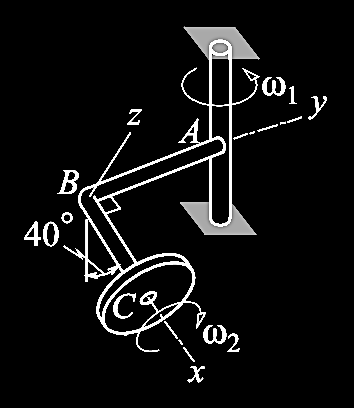
\includegraphics[frame]{images/Q3_28.png}
\end{figure}}

\subsubsection*{(a) Describe the angular velocity of the rotor in terms of a superposition of simple rotations.}

Construct the angular velocity vector $\bar{\omega}$ of $xyz$ by vectorially adding the simple rotation rates according to:

$$ \bar{\omega} = \omega_1 \bar{e}_1 + \omega_2 \bar{e}_2$$

This gives us:

$$ \bar{\omega} = \omega_1 \bar{K} + \omega_2 (-\bar{i})$$

Or:

\begin{answer}
$$ \bar{\omega} = \omega_1 \bar{K} +  \omega_2 \bar{i}$$
\end{answer}

\subsubsection*{(b) Solely from an examination of the description in Part (a), predict the direction(s) in which the angular acceleration of the rotor will be situated relative to the xyz axes defined in the sketch. Briefly explain your answer.}

Sketching this out the frames relative to each other:

\begin{center}
\tikzset{
pattern size/.store in=\mcSize, 
pattern size = 5pt,
pattern thickness/.store in=\mcThickness, 
pattern thickness = 0.3pt,
pattern radius/.store in=\mcRadius, 
pattern radius = 1pt}
\makeatletter
\pgfutil@ifundefined{pgf@pattern@name@_3f955ijae}{
\pgfdeclarepatternformonly[\mcThickness,\mcSize]{_3f955ijae}
{\pgfqpoint{-\mcThickness}{-\mcThickness}}
{\pgfpoint{\mcSize}{\mcSize}}
{\pgfpoint{\mcSize}{\mcSize}}
{
\pgfsetcolor{\tikz@pattern@color}
\pgfsetlinewidth{\mcThickness}
\pgfpathmoveto{\pgfpointorigin}
\pgfpathlineto{\pgfpoint{0}{\mcSize}}
\pgfusepath{stroke}
}}
\makeatother

% Pattern Info
 
\tikzset{
pattern size/.store in=\mcSize, 
pattern size = 5pt,
pattern thickness/.store in=\mcThickness, 
pattern thickness = 0.3pt,
pattern radius/.store in=\mcRadius, 
pattern radius = 1pt}
\makeatletter
\pgfutil@ifundefined{pgf@pattern@name@_6pdewzxwt}{
\pgfdeclarepatternformonly[\mcThickness,\mcSize]{_6pdewzxwt}
{\pgfqpoint{-\mcThickness}{-\mcThickness}}
{\pgfpoint{\mcSize}{\mcSize}}
{\pgfpoint{\mcSize}{\mcSize}}
{
\pgfsetcolor{\tikz@pattern@color}
\pgfsetlinewidth{\mcThickness}
\pgfpathmoveto{\pgfpointorigin}
\pgfpathlineto{\pgfpoint{0}{\mcSize}}
\pgfusepath{stroke}
}}
\makeatother
\tikzset{every picture/.style={line width=0.75pt}} %set default line width to 0.75pt        

\begin{tikzpicture}[x=0.75pt,y=0.75pt,yscale=-1,xscale=1]
%uncomment if require: \path (0,269); %set diagram left start at 0, and has height of 269

%Straight Lines [id:da20435224588937562] 
\draw [line width=1.5]    (314,151) -- (315,61) ;
%Straight Lines [id:da03445781531687486] 
\draw    (314,151) -- (411,152) ;
%Straight Lines [id:da7893099740949647] 
\draw [line width=0.75]    (358,85) -- (314,151) ;
%Straight Lines [id:da8958798831337074] 
\draw [line width=0.75]    (314,151) -- (366,225) ;
%Straight Lines [id:da3609400739420203] 
\draw [pattern=_3f955ijae,pattern size=6pt,pattern thickness=0.75pt,pattern radius=0pt, pattern color={rgb, 255:red, 0; green, 0; blue, 0}][line width=0.75]  [dash pattern={on 4.5pt off 4.5pt}]  (314,151) -- (315,241) ;
%Curve Lines [id:da8730659221398798] 
\draw    (336,118) .. controls (334,101) and (318,103) .. (314.5,106) ;
%Curve Lines [id:da41577213022532145] 
\draw    (314.5,196) .. controls (324.5,204) and (341,186) .. (336,182) ;
%Straight Lines [id:da6094981848974355] 
\draw [pattern=_6pdewzxwt,pattern size=6pt,pattern thickness=0.75pt,pattern radius=0pt, pattern color={rgb, 255:red, 0; green, 0; blue, 0}][line width=0.75]  [dash pattern={on 4.5pt off 4.5pt}]  (314,151) -- (276,87) ;
%Curve Lines [id:da6552705712368743] 
\draw    (314.5,106) .. controls (300,101.5) and (295.5,110) .. (292,113) ;

% Text Node
\draw (366,220) node [anchor=north west][inner sep=0.75pt]   [align=left] {$x$};
% Text Node
\draw (414.54,143.31) node [anchor=north west][inner sep=0.75pt]   [align=left] {$y$};
% Text Node
\draw (360,68) node [anchor=north west][inner sep=0.75pt]   [align=left] {$z$};
% Text Node
\draw (308,43) node [anchor=north west][inner sep=0.75pt]   [align=left] {$Z$};
% Text Node
\draw (298,144) node [anchor=north west][inner sep=0.75pt]   [align=left] {$C$};
% Text Node
\draw (313.5,177) node [anchor=north west][inner sep=0.75pt]   [align=left] {{\scriptsize $40^\circ$}};
% Text Node
\draw (315.0,109) node [anchor=north west][inner sep=0.75pt]   [align=left] {{\scriptsize $50^\circ$}};
% Text Node
\draw (295.5,107) node [anchor=north west][inner sep=0.75pt]   [align=left] {{\scriptsize $40^\circ$}};

\end{tikzpicture}
\end{center}

\subsubsection*{(c) Describe the angular velocity and angular acceleration of the rotor in terms of components relative to xyz.}

Because the first auxiliary reference frame is stationary, and the second one is $xyz$, we have:

$$ \bar{\Omega}_1 = \bar{0}, \ \ \bar{\Omega}_2 = \bar{\omega} $$

We find the global components of the unit vectors by inspection of the sketch, which leads to

\begin{equation*}
\begin{aligned}
\bar{K} &= \cos(40^\circ)(-\hat{i}) + \cos(50^\circ)\hat{k} \\
        &= -\cos(40^\circ)\hat{i} + \cos(50^\circ)\hat{k}  \\
\bar{i} &= \hat{i} 
\end{aligned}
\end{equation*}

This makes the velocity:

\begin{answer}
$$ \bar{\omega} = \left(\omega_2-\cos(40^\circ)\omega_1\right) \hat{i} + \omega_1\cos(50^\circ)\hat{k} $$
\end{answer}

Next solve for angular acceleration:

$$ \bar{\alpha} =
\sum_n \left( \dot{\omega}_n \bar{e}_n + \bar{\Omega}_n \times \omega_n \bar{e}_n \right) $$

Since $n=2$:

$$ \bar{\alpha} =
\dot{\omega}_1 \bar{e}_1 + \bar{\Omega}_1 \times \omega_1 \bar{e}_1 +
\dot{\omega}_2 \bar{e}_2 + \bar{\Omega}_2 \times \omega_2 \bar{e}_2 $$

And since $\dot{\omega}_1 = \dot{\omega}_2 = 0$:

$$ \bar{\alpha} =
\bar{\Omega}_1 \times \omega_1 \bar{e}_1 +
\bar{\Omega}_2 \times \omega_2 \bar{e}_2 $$

Futher, as stated above that $\bar{\Omega}_1 = \bar{0}$ and $\bar{\Omega}_2 = \bar{\omega}$:

\begin{equation*}
\begin{aligned}
\bar{\alpha} &= \bar{\Omega}_2 \times \omega_2 \bar{e}_2\\
             &= \left( \left(\omega_2-\cos(40^\circ)\omega_1\right) \hat{i} + \omega_1\cos(50^\circ)\hat{k} \right)
                \times \omega_2 (-i)\\
            &= -\omega_2 \left( \left(\omega_2-\cos(40^\circ)\omega_1\right) \hat{i} + \omega_1\cos(50^\circ)\hat{k} \right)
                \times i\\
\end{aligned}
\end{equation*}

Which solves to:

\begin{answer}
$$ \bar{\alpha} = -\omega_1 \omega_2 \cos(50^\circ) \hat{j} $$
\end{answer}

\subsection*{EXERCISE 3.37}
\subsubsection*{The angle $\bm{\theta}$ describing the rotation of a reconnaissance satellite's solar panels about the body-fixed $\bm{x}$ axis is an arbitrary function of time.
The satellite spins about the $\bm{z}$ axis at the constant rate $\bm{\Omega}$.
Derive expressions for the absolute velocity and acceleration of point $\bm{B}$ relative to the origin of $\bm{xyz}$.
\begin{figure}[H]
    \centering
    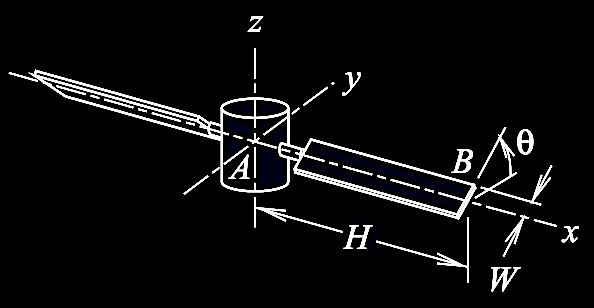
\includegraphics[frame]{images/Q3_37.png}
\end{figure}}

Construct the angular velocity vector $\bar{\omega}$ of $xyz$ by vectorially adding the simple rotation rates according to:

$$ \bar{\omega} = \omega_1 \bar{e}_1 + \omega_2 \bar{e}_2$$

This gives us:

$$ \bar{\omega} = \Omega\ \bar{k}' + \dot{\theta}\ \bar{i}'$$

Next solve for angular acceleration:

$$ \bar{\alpha} =
\sum_n \left( \dot{\omega}_n \bar{e}_n + \bar{\Omega}_n \times \omega_n \bar{e}_n \right) $$

Since $n=2$:

$$ \bar{\alpha} =
\dot{\omega}_1 \bar{e}_1 + \bar{\Omega}_1 \times \omega_1 \bar{e}_1 +
\dot{\omega}_2 \bar{e}_2 + \bar{\Omega}_2 \times \omega_2 \bar{e}_2 $$

And since $\dot{\omega}_1 = \dot{\omega}_2 = 0$:

$$ \bar{\alpha} =
\bar{\Omega}_1 \times \omega_1 \bar{e}_1 +
\bar{\Omega}_2 \times \omega_2 \bar{e}_2 $$

Since, as stated above that $\bar{\Omega}_1 = \Omega \bar{k}'$ and $\bar{\Omega}_2 = \bar{\omega}$:

\begin{equation*}
\begin{aligned}
\bar{\alpha} &= \Omega \hat{k} \times \Omega \hat{k} + \left( \Omega\ \hat{k} + \dot{\theta}\ \hat{i} \right) \times \theta \hat{i} \\
             &= \Omega \theta \hat{j}
\end{aligned}
\end{equation*}

% \color{white}
% \hspace*{6em}\inputminted[frame=leftline,fontsize=\footnotesize]{matlab}
% {./matlab/B_2_18.m}
% \color{black} 

% It has the following response, which matches my analytically derived solution:

% \begin{figure}[H]
%     \centering
%     \includegraphics{matlab/B_2_18.png}
%     \caption{Response of the system}
% \end{figure}

\end{document}

